\documentclass[crop,tikz,convert={outext=.svg,command=\unexpanded{pdf2svg \infile\space\outfile}},multi=false]{standalone}[2012/04/13]
%\usetikzlibrary{...}% tikz package already loaded by 'tikz' option
\makeatletter
\begin{document}% Created by tikzDevice version 0.12.3 on 2019-09-06 10:09:11
	% !TEX encoding = UTF-8 Unicode
	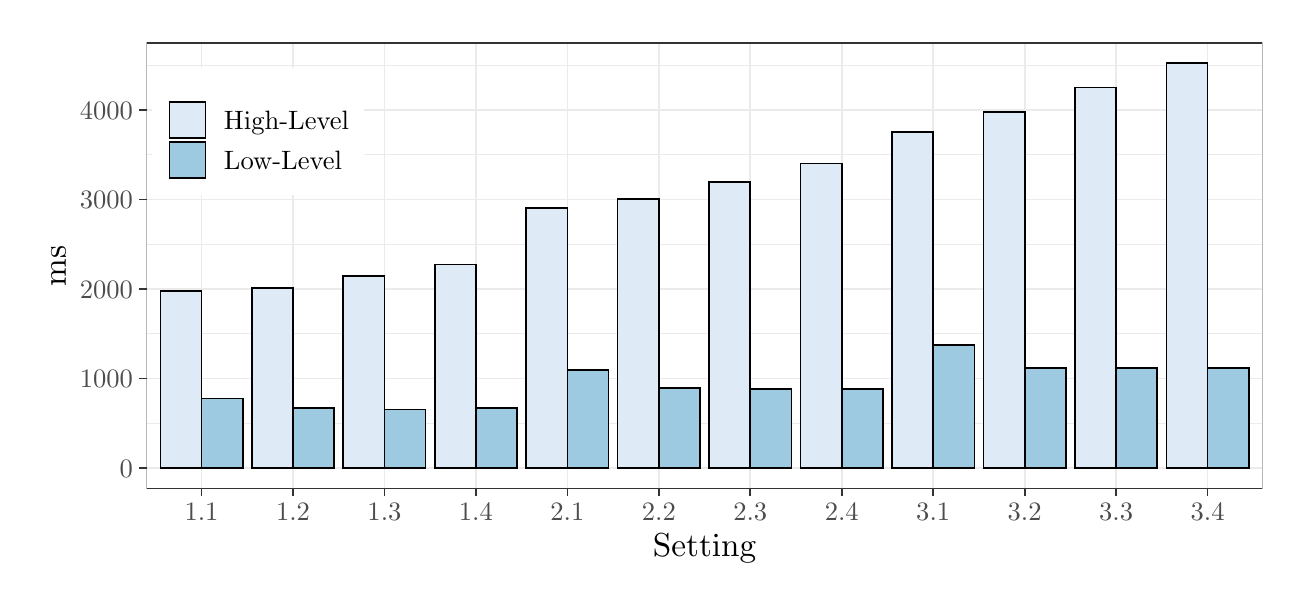
\begin{tikzpicture}[x=1pt,y=1pt]
	\definecolor{fillColor}{RGB}{255,255,255}
	\path[use as bounding box,fill=fillColor,fill opacity=0.00] (0,0) rectangle (451.69,198.74);
	\begin{scope}
	\path[clip] (  0.00,  0.00) rectangle (451.69,198.74);
	\definecolor{drawColor}{RGB}{255,255,255}
	\definecolor{fillColor}{RGB}{255,255,255}
	
	\path[draw=drawColor,line width= 0.6pt,line join=round,line cap=round,fill=fillColor] (  0.00,  0.00) rectangle (451.69,198.74);
	\end{scope}
	\begin{scope}
	\path[clip] ( 42.99, 32.28) rectangle (446.19,193.24);
	\definecolor{fillColor}{RGB}{255,255,255}
	
	\path[fill=fillColor] ( 42.99, 32.28) rectangle (446.19,193.24);
	\definecolor{drawColor}{gray}{0.92}
	
	\path[draw=drawColor,line width= 0.3pt,line join=round] ( 42.99, 55.76) --
	(446.19, 55.76);
	
	\path[draw=drawColor,line width= 0.3pt,line join=round] ( 42.99, 88.10) --
	(446.19, 88.10);
	
	\path[draw=drawColor,line width= 0.3pt,line join=round] ( 42.99,120.44) --
	(446.19,120.44);
	
	\path[draw=drawColor,line width= 0.3pt,line join=round] ( 42.99,152.77) --
	(446.19,152.77);
	
	\path[draw=drawColor,line width= 0.3pt,line join=round] ( 42.99,185.11) --
	(446.19,185.11);
	
	\path[draw=drawColor,line width= 0.6pt,line join=round] ( 42.99, 39.59) --
	(446.19, 39.59);
	
	\path[draw=drawColor,line width= 0.6pt,line join=round] ( 42.99, 71.93) --
	(446.19, 71.93);
	
	\path[draw=drawColor,line width= 0.6pt,line join=round] ( 42.99,104.27) --
	(446.19,104.27);
	
	\path[draw=drawColor,line width= 0.6pt,line join=round] ( 42.99,136.60) --
	(446.19,136.60);
	
	\path[draw=drawColor,line width= 0.6pt,line join=round] ( 42.99,168.94) --
	(446.19,168.94);
	
	\path[draw=drawColor,line width= 0.6pt,line join=round] ( 62.82, 32.28) --
	( 62.82,193.24);
	
	\path[draw=drawColor,line width= 0.6pt,line join=round] ( 95.87, 32.28) --
	( 95.87,193.24);
	
	\path[draw=drawColor,line width= 0.6pt,line join=round] (128.92, 32.28) --
	(128.92,193.24);
	
	\path[draw=drawColor,line width= 0.6pt,line join=round] (161.97, 32.28) --
	(161.97,193.24);
	
	\path[draw=drawColor,line width= 0.6pt,line join=round] (195.02, 32.28) --
	(195.02,193.24);
	
	\path[draw=drawColor,line width= 0.6pt,line join=round] (228.07, 32.28) --
	(228.07,193.24);
	
	\path[draw=drawColor,line width= 0.6pt,line join=round] (261.11, 32.28) --
	(261.11,193.24);
	
	\path[draw=drawColor,line width= 0.6pt,line join=round] (294.16, 32.28) --
	(294.16,193.24);
	
	\path[draw=drawColor,line width= 0.6pt,line join=round] (327.21, 32.28) --
	(327.21,193.24);
	
	\path[draw=drawColor,line width= 0.6pt,line join=round] (360.26, 32.28) --
	(360.26,193.24);
	
	\path[draw=drawColor,line width= 0.6pt,line join=round] (393.31, 32.28) --
	(393.31,193.24);
	
	\path[draw=drawColor,line width= 0.6pt,line join=round] (426.36, 32.28) --
	(426.36,193.24);
	\definecolor{drawColor}{RGB}{0,0,0}
	\definecolor{fillColor}{RGB}{158,202,225}
	
	\path[draw=drawColor,line width= 0.6pt,line cap=rect,fill=fillColor] ( 62.82, 39.59) rectangle ( 77.69, 64.80);
	\definecolor{fillColor}{RGB}{222,235,247}
	
	\path[draw=drawColor,line width= 0.6pt,line cap=rect,fill=fillColor] ( 47.95, 39.59) rectangle ( 62.82,103.68);
	\definecolor{fillColor}{RGB}{158,202,225}
	
	\path[draw=drawColor,line width= 0.6pt,line cap=rect,fill=fillColor] ( 95.87, 39.59) rectangle (110.74, 61.37);
	\definecolor{fillColor}{RGB}{222,235,247}
	
	\path[draw=drawColor,line width= 0.6pt,line cap=rect,fill=fillColor] ( 81.00, 39.59) rectangle ( 95.87,104.75);
	\definecolor{fillColor}{RGB}{158,202,225}
	
	\path[draw=drawColor,line width= 0.6pt,line cap=rect,fill=fillColor] (128.92, 39.59) rectangle (143.79, 60.75);
	\definecolor{fillColor}{RGB}{222,235,247}
	
	\path[draw=drawColor,line width= 0.6pt,line cap=rect,fill=fillColor] (114.05, 39.59) rectangle (128.92,109.03);
	\definecolor{fillColor}{RGB}{158,202,225}
	
	\path[draw=drawColor,line width= 0.6pt,line cap=rect,fill=fillColor] (161.97, 39.59) rectangle (176.84, 61.29);
	\definecolor{fillColor}{RGB}{222,235,247}
	
	\path[draw=drawColor,line width= 0.6pt,line cap=rect,fill=fillColor] (147.10, 39.59) rectangle (161.97,113.10);
	\definecolor{fillColor}{RGB}{158,202,225}
	
	\path[draw=drawColor,line width= 0.6pt,line cap=rect,fill=fillColor] (195.02, 39.59) rectangle (209.89, 74.94);
	\definecolor{fillColor}{RGB}{222,235,247}
	
	\path[draw=drawColor,line width= 0.6pt,line cap=rect,fill=fillColor] (180.15, 39.59) rectangle (195.02,133.48);
	\definecolor{fillColor}{RGB}{158,202,225}
	
	\path[draw=drawColor,line width= 0.6pt,line cap=rect,fill=fillColor] (228.07, 39.59) rectangle (242.94, 68.62);
	\definecolor{fillColor}{RGB}{222,235,247}
	
	\path[draw=drawColor,line width= 0.6pt,line cap=rect,fill=fillColor] (213.19, 39.59) rectangle (228.07,136.90);
	\definecolor{fillColor}{RGB}{158,202,225}
	
	\path[draw=drawColor,line width= 0.6pt,line cap=rect,fill=fillColor] (261.11, 39.59) rectangle (275.99, 68.15);
	\definecolor{fillColor}{RGB}{222,235,247}
	
	\path[draw=drawColor,line width= 0.6pt,line cap=rect,fill=fillColor] (246.24, 39.59) rectangle (261.11,142.91);
	\definecolor{fillColor}{RGB}{158,202,225}
	
	\path[draw=drawColor,line width= 0.6pt,line cap=rect,fill=fillColor] (294.16, 39.59) rectangle (309.04, 68.21);
	\definecolor{fillColor}{RGB}{222,235,247}
	
	\path[draw=drawColor,line width= 0.6pt,line cap=rect,fill=fillColor] (279.29, 39.59) rectangle (294.16,149.65);
	\definecolor{fillColor}{RGB}{158,202,225}
	
	\path[draw=drawColor,line width= 0.6pt,line cap=rect,fill=fillColor] (327.21, 39.59) rectangle (342.08, 84.01);
	\definecolor{fillColor}{RGB}{222,235,247}
	
	\path[draw=drawColor,line width= 0.6pt,line cap=rect,fill=fillColor] (312.34, 39.59) rectangle (327.21,161.12);
	\definecolor{fillColor}{RGB}{158,202,225}
	
	\path[draw=drawColor,line width= 0.6pt,line cap=rect,fill=fillColor] (360.26, 39.59) rectangle (375.13, 75.84);
	\definecolor{fillColor}{RGB}{222,235,247}
	
	\path[draw=drawColor,line width= 0.6pt,line cap=rect,fill=fillColor] (345.39, 39.59) rectangle (360.26,168.21);
	\definecolor{fillColor}{RGB}{158,202,225}
	
	\path[draw=drawColor,line width= 0.6pt,line cap=rect,fill=fillColor] (393.31, 39.59) rectangle (408.18, 75.75);
	\definecolor{fillColor}{RGB}{222,235,247}
	
	\path[draw=drawColor,line width= 0.6pt,line cap=rect,fill=fillColor] (378.44, 39.59) rectangle (393.31,177.07);
	\definecolor{fillColor}{RGB}{158,202,225}
	
	\path[draw=drawColor,line width= 0.6pt,line cap=rect,fill=fillColor] (426.36, 39.59) rectangle (441.23, 75.87);
	\definecolor{fillColor}{RGB}{222,235,247}
	
	\path[draw=drawColor,line width= 0.6pt,line cap=rect,fill=fillColor] (411.49, 39.59) rectangle (426.36,185.93);
	\definecolor{drawColor}{gray}{0.20}
	
	\path[draw=drawColor,line width= 0.6pt,line join=round,line cap=round] ( 42.99, 32.28) rectangle (446.19,193.24);
	\end{scope}
	\begin{scope}
	\path[clip] (  0.00,  0.00) rectangle (451.69,198.74);
	\definecolor{drawColor}{gray}{0.30}
	
	\node[text=drawColor,anchor=base east,inner sep=0pt, outer sep=0pt, scale=  0.96] at ( 38.04, 36.29) {0};
	
	\node[text=drawColor,anchor=base east,inner sep=0pt, outer sep=0pt, scale=  0.96] at ( 38.04, 68.62) {1000};
	
	\node[text=drawColor,anchor=base east,inner sep=0pt, outer sep=0pt, scale=  0.96] at ( 38.04,100.96) {2000};
	
	\node[text=drawColor,anchor=base east,inner sep=0pt, outer sep=0pt, scale=  0.96] at ( 38.04,133.30) {3000};
	
	\node[text=drawColor,anchor=base east,inner sep=0pt, outer sep=0pt, scale=  0.96] at ( 38.04,165.64) {4000};
	\end{scope}
	\begin{scope}
	\path[clip] (  0.00,  0.00) rectangle (451.69,198.74);
	\definecolor{drawColor}{gray}{0.20}
	
	\path[draw=drawColor,line width= 0.6pt,line join=round] ( 40.24, 39.59) --
	( 42.99, 39.59);
	
	\path[draw=drawColor,line width= 0.6pt,line join=round] ( 40.24, 71.93) --
	( 42.99, 71.93);
	
	\path[draw=drawColor,line width= 0.6pt,line join=round] ( 40.24,104.27) --
	( 42.99,104.27);
	
	\path[draw=drawColor,line width= 0.6pt,line join=round] ( 40.24,136.60) --
	( 42.99,136.60);
	
	\path[draw=drawColor,line width= 0.6pt,line join=round] ( 40.24,168.94) --
	( 42.99,168.94);
	\end{scope}
	\begin{scope}
	\path[clip] (  0.00,  0.00) rectangle (451.69,198.74);
	\definecolor{drawColor}{gray}{0.20}
	
	\path[draw=drawColor,line width= 0.6pt,line join=round] ( 62.82, 29.53) --
	( 62.82, 32.28);
	
	\path[draw=drawColor,line width= 0.6pt,line join=round] ( 95.87, 29.53) --
	( 95.87, 32.28);
	
	\path[draw=drawColor,line width= 0.6pt,line join=round] (128.92, 29.53) --
	(128.92, 32.28);
	
	\path[draw=drawColor,line width= 0.6pt,line join=round] (161.97, 29.53) --
	(161.97, 32.28);
	
	\path[draw=drawColor,line width= 0.6pt,line join=round] (195.02, 29.53) --
	(195.02, 32.28);
	
	\path[draw=drawColor,line width= 0.6pt,line join=round] (228.07, 29.53) --
	(228.07, 32.28);
	
	\path[draw=drawColor,line width= 0.6pt,line join=round] (261.11, 29.53) --
	(261.11, 32.28);
	
	\path[draw=drawColor,line width= 0.6pt,line join=round] (294.16, 29.53) --
	(294.16, 32.28);
	
	\path[draw=drawColor,line width= 0.6pt,line join=round] (327.21, 29.53) --
	(327.21, 32.28);
	
	\path[draw=drawColor,line width= 0.6pt,line join=round] (360.26, 29.53) --
	(360.26, 32.28);
	
	\path[draw=drawColor,line width= 0.6pt,line join=round] (393.31, 29.53) --
	(393.31, 32.28);
	
	\path[draw=drawColor,line width= 0.6pt,line join=round] (426.36, 29.53) --
	(426.36, 32.28);
	\end{scope}
	\begin{scope}
	\path[clip] (  0.00,  0.00) rectangle (451.69,198.74);
	\definecolor{drawColor}{gray}{0.30}
	
	\node[text=drawColor,anchor=base,inner sep=0pt, outer sep=0pt, scale=  0.96] at ( 62.82, 20.71) {1.1};
	
	\node[text=drawColor,anchor=base,inner sep=0pt, outer sep=0pt, scale=  0.96] at ( 95.87, 20.71) {1.2};
	
	\node[text=drawColor,anchor=base,inner sep=0pt, outer sep=0pt, scale=  0.96] at (128.92, 20.71) {1.3};
	
	\node[text=drawColor,anchor=base,inner sep=0pt, outer sep=0pt, scale=  0.96] at (161.97, 20.71) {1.4};
	
	\node[text=drawColor,anchor=base,inner sep=0pt, outer sep=0pt, scale=  0.96] at (195.02, 20.71) {2.1};
	
	\node[text=drawColor,anchor=base,inner sep=0pt, outer sep=0pt, scale=  0.96] at (228.07, 20.71) {2.2};
	
	\node[text=drawColor,anchor=base,inner sep=0pt, outer sep=0pt, scale=  0.96] at (261.11, 20.71) {2.3};
	
	\node[text=drawColor,anchor=base,inner sep=0pt, outer sep=0pt, scale=  0.96] at (294.16, 20.71) {2.4};
	
	\node[text=drawColor,anchor=base,inner sep=0pt, outer sep=0pt, scale=  0.96] at (327.21, 20.71) {3.1};
	
	\node[text=drawColor,anchor=base,inner sep=0pt, outer sep=0pt, scale=  0.96] at (360.26, 20.71) {3.2};
	
	\node[text=drawColor,anchor=base,inner sep=0pt, outer sep=0pt, scale=  0.96] at (393.31, 20.71) {3.3};
	
	\node[text=drawColor,anchor=base,inner sep=0pt, outer sep=0pt, scale=  0.96] at (426.36, 20.71) {3.4};
	\end{scope}
	\begin{scope}
	\path[clip] (  0.00,  0.00) rectangle (451.69,198.74);
	\definecolor{drawColor}{RGB}{0,0,0}
	
	\node[text=drawColor,anchor=base,inner sep=0pt, outer sep=0pt, scale=  1.20] at (244.59,  7.83) {Setting};
	\end{scope}
	\begin{scope}
	\path[clip] (  0.00,  0.00) rectangle (451.69,198.74);
	\definecolor{drawColor}{RGB}{0,0,0}
	
	\node[text=drawColor,rotate= 90.00,anchor=base,inner sep=0pt, outer sep=0pt, scale=  1.20] at ( 13.76,112.76) {ms};
	\end{scope}
	\begin{scope}
	\path[clip] (  0.00,  0.00) rectangle (451.69,198.74);
	\definecolor{fillColor}{RGB}{255,255,255}
	
	\path[fill=fillColor] ( 44.99,138.10) rectangle (121.63,184.00);
	\end{scope}
	\begin{scope}
	\path[clip] (  0.00,  0.00) rectangle (451.69,198.74);
	\definecolor{fillColor}{RGB}{255,255,255}
	
	\path[fill=fillColor] ( 50.49,158.05) rectangle ( 64.94,172.50);
	\end{scope}
	\begin{scope}
	\path[clip] (  0.00,  0.00) rectangle (451.69,198.74);
	\definecolor{drawColor}{RGB}{0,0,0}
	\definecolor{fillColor}{RGB}{222,235,247}
	
	\path[draw=drawColor,line width= 0.6pt,line cap=rect,fill=fillColor] ( 51.20,158.76) rectangle ( 64.23,171.79);
	\end{scope}
	\begin{scope}
	\path[clip] (  0.00,  0.00) rectangle (451.69,198.74);
	\definecolor{fillColor}{RGB}{255,255,255}
	
	\path[fill=fillColor] ( 50.49,143.60) rectangle ( 64.94,158.05);
	\end{scope}
	\begin{scope}
	\path[clip] (  0.00,  0.00) rectangle (451.69,198.74);
	\definecolor{drawColor}{RGB}{0,0,0}
	\definecolor{fillColor}{RGB}{158,202,225}
	
	\path[draw=drawColor,line width= 0.6pt,line cap=rect,fill=fillColor] ( 51.20,144.31) rectangle ( 64.23,157.34);
	\end{scope}
	\begin{scope}
	\path[clip] (  0.00,  0.00) rectangle (451.69,198.74);
	\definecolor{drawColor}{RGB}{0,0,0}
	
	\node[text=drawColor,anchor=base west,inner sep=0pt, outer sep=0pt, scale=  0.96] at ( 70.94,161.97) {High-Level};
	\end{scope}
	\begin{scope}
	\path[clip] (  0.00,  0.00) rectangle (451.69,198.74);
	\definecolor{drawColor}{RGB}{0,0,0}
	
	\node[text=drawColor,anchor=base west,inner sep=0pt, outer sep=0pt, scale=  0.96] at ( 70.94,147.52) {Low-Level};
	\end{scope}
	\end{tikzpicture}
\end{document}